\scanpage{98}
Donc il s'ensuit que $M_3\deleted{\unsure{[1/3]}}\cap V(c_4)$ a exactement 4 composantes irréductibles, \deleted{\unsure{elles}} qui ne peuvent se rencontrer qu'au dessus du point $p=2$. Il y a \unsure{évidemt} 1 composantes connexes, car la fibre de $M_3[1/3]$ au dessus de l'unique point de $\mu_3^*$ sur $p=2$ [qui correspond au \deleted{\unsure{$\mathbb F$}} corps résiduel $\mathbb F_4=\mathbb F_2(\sqrt[3]{1})$] est de \deleted{degré} rang géom. 1. Cela provient du fait que le \unsure{gpe} des \unsure{autom.} d'une \unsure{c.} $E$ en car. 2 \inserted{(sur corps alg clos)} avec $c_4=0$, est $\mathrm{Sl}(2,\mathbb Z/3\mathbb Z)$, \deleted{qui agit \unsure{transitivement} sur l'ens des \unsure{toutes} les bases}\inserted{et l'\unsure{ens|aire|une} des orbites sous ce groupe de l'ens des \deleted{toutes} les} bases de $\mathord{}_3E$ est deux.

\figure{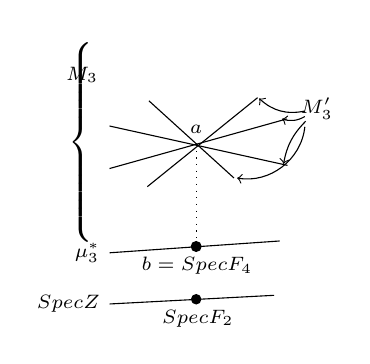
\begin{tikzpicture}[x=1cm,y=1cm,font=\scriptsize]
\node at (-.35,3.15) {$M_3$}; \node at (-.35,2.33) {\(\left\{\rule{0pt}{1.4cm}\right.\)};
\draw (0,1.96)--(2.25,2.59); \draw (0,2.50)--(2.26,2.00);
\draw (.48,1.73)--(1.88,2.86); \draw (.50,2.82)--(1.58,1.84);
\node[above] at (1.1,2.28) {$a$};
\node at (2.63,2.72) {$M'_3$};
\draw[->] (2.48,2.69) to[bend left=27] (1.90,2.85);
\draw[->] (2.48,2.62) to[bend left=23] (2.19,2.59);
\draw[->] (2.49,2.56) to[bend right=17] (2.21,2.02);
\draw[->] (2.48,2.49) to[bend left=47] (1.62,1.84);
\draw[dotted] (1.10,2.27)--(1.10,.93);
\draw (0,.89)--(2.16,1.04); \fill (1.10,.97) circle (2pt);
\node[left] at (0,.89) {$\mu_3^*$}; \node[below] at (1.11,.96) {$b=\operatorname{Spec}\mathbb F_4$};
\draw (0,.24)--(2.09,.35); \fill (1.10,.30) circle (1.9pt);
\node[left] at (0,.24) {$\operatorname{Spec}\mathbb Z$}; \node[below] at (1.12,.29) {$\operatorname{Spec}\mathbb F_2$};
\end{tikzpicture}}

\deleted{\unsure{qui sont}} La courbe $\unsure{\mathbb E|E|\overline E}$ \deleted{\unsure{se descend évidemment}}\inserted{a bonne réduction} sur \inserted{tout} l'anneau des entiers \deleted{\unsure{des}} corps de $\mu_3^*$, \unsure{ou|sur} $\mathbb Q(\sqrt[3]{1})$, \deleted{Il y a} sans exclure 2 (ni 3 ?). Comme $\deleted{\unsure{V'}}M_3^{\unsure{*|2}}\deleted{\unsure{[1/3]}}$ et à fortiori $M_3\cap V(c_4)$ est au dessus de $\mu_3^*[\frac13]$, il s'ensuit que les composantes irréductibles (qui sont entières sur $\mu_3^*[\frac13]$ et \unsure{birationelles|birationnelles} sur lui) sont \uline{identiques} à $\mu_3^*[\frac13]$. Donc chacune des \unsure{restrictions} de la courbe \inserted{elliptique} universelle sur $M_3$ aux composantes irréductibles de $\mu_3^*[\frac13]$ sont isomorphes à $\mathbb E$ envisagé plus haut (ou plutôt, son extension canonique à $\mu_3^*[\frac13]$ -- on voit qu'elles se réduisent bien aussi au point $p=2$), mais avec des 3-rigidifications différentes. Le raccord des quatre composantes se fait d'abord \unsure{$\circ$}
% slanted
\margin{\unsure{$\circ$} grâce au fait que les fibres de \unsure{ces} $E^{(i)}$ en $a$ \unsure{s.t|st|et à} (de façon unique) isomorphes comme courbes elliptiques \uline{rig.} d'échelon 3 ; mais le \unsure{raccordement|raisonnement|raccord|second énoncé} est encore trop lâche \ldots\ldots}

A examiner si les \deleted{tangentes} 4 composantes de $M'_3$ en le point $a$ de $(M'_3)_2$ \deleted{sont} ``à tangentes distinctes'' ; comme le corps résiduel est $\mathbb F_4$, et que $\operatorname{card}\mathbb P^1_{\mathbb F_4}=5$, dont il faut enlever la verticale, cela \uline{signifierait} que les tangentes épuisent toutes les classes non verticales de l'espace tangent de Zariski en $a$. Or ces tangentes sont transformées \inserted{l'une de l'autre} par \unsure{l'opérations|les opérations} de $G'=\mathrm{Sl}(2,\mathbb Z_{/3\mathbb Z})$. [qui est le \unsure{un} groupe d'inertie \unsure{du|en} $a$, est un groupe de \deleted{\unsure{$\mathbb F$ ou}} \unsure{$\mu_3^*\!{}_{T_a}$-autom|$\mu'_3$-autom} de] \deleted{le groupe qui laisse} Comment opère-t-il sur l'espace tangent de Zariski \inserted{de} en $a$ ? \deleted{qui} Il doit laisser invariant l'application $T_a\to T_b$, \deleted{donc le} (car op. trivialemt sur $T_b$) donc opère via $\mathbb F_4^*\cdot\mathbb F_4$.
\margin{sur $\unsure{\mathbb F_3|\mathbb F_4}$ \quad $\begin{pmatrix}*&*\\0&1\end{pmatrix}$}
Notons que $B'$ \deleted{\unsure{opè}} laisse chaque composante irréductible invariante, donc \deleted{laisse invariante leurs \unsure{espaces}}\inserted{opère trivialemt, donc opère} \deleted{\unsure{sur}} \inserted{trivialt sur l'espace} \deleted{tangent} de Zariski ; \deleted{donc $B'$ opère} s'il y en avait deux distinctes, il opérerait aussi trivialement sur l'espace tangent de Zariski de $M_3$ en $a$, mais alors (comme le ss. gpe inv. de $G'$ engendré par $B'$ est $G'$) \deleted{$G'$ \unsure{est}} \deleted{il \unsure{engendrerait}} opérant trivialement, et comme il est transitif] sur l'ens des tangentes des composantes de $M'_3$ en $a$, on aurait contradiction. \uline{Donc les quatre}
% archive sheet number: 97
